\documentclass[10pt,a4paper]{article}
\usepackage[utf8]{inputenc}
\usepackage[spanish]{babel}
\usepackage{amsmath}
\usepackage{amsfonts}
\usepackage{amssymb}
\usepackage{graphicx}
\usepackage[hidelinks]{hyperref}
\usepackage{listings}
\usepackage[left=2cm,right=2cm,top=2cm,bottom=2cm]{geometry}

\lstset { frame = single, breaklines = true }

\begin{document}

\begin{titlepage}
\title{\textbf{
	{\Huge Encapsular el acceso a una aplicación BASIC/MS-DOS}\\
	{\Large Sistemas Legados}
}}
\author{
	Pedro Allué Tamargo (758267)
	\and
	Juan José Tambo Tambo (755742)
	\and
	Jesús Villacampa Sagaste (755739)
}
\date{\today}
\clearpage\maketitle
\thispagestyle{empty}
\tableofcontents
\end{titlepage}


\section{Introducción}

En esta práctica se pide la realización de un \emph{wrapper} sobre una aplicación legada de un sistema \emph{MS-DOS}. Para ello se va a utilizar un emulador y mediante capturas de pantallas de la interacción con la misma y un software de reconocimiento de caracteres (\emph{OCR}) se van a extraer los datos.


\section{Esfuerzos invertidos}

\begin{itemize}
\item Pedro Allué Tamargo: Creación de la API REST, organización de la estructura de proyectos, implementación de la clase \emph{Wrapper}, redacción de la memoria.
	\begin{itemize}
	\item Tiempo invertido: 10 horas
	\end{itemize}
\item Juan José Tambo Tambo:
\item Jesús Villacampa Sagaste:
\end{itemize}

\section{Descripción de la aplicación legada}

Para interaccionar con la aplicación legada se va a utilizar el emulador \emph{DosBox} (el incluido junto al enunciado de la práctica). Para ejecutar la aplicación se va a ejecutar el \emph{script} \texttt{database.bat} que ejecuta el emulador y la aplicación legada.\\
La aplicación legada consiste en un programa de \emph{MS-DOS} que gestiona una biblioteca de cintas con distintos programas y/o juegos (Figura \ref{fig:aplicacion_legada}).

\begin{figure}[h!]
\centering
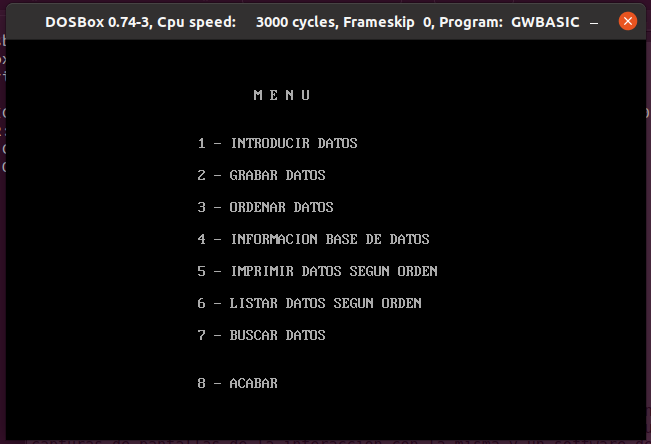
\includegraphics[scale=0.5]{images/aplicacion_legada.png}
\caption{Captura de pantalla del menú principal de la aplicación legada}
\label{fig:aplicacion_legada}
\end{figure}

Con esta aplicación el usuario podía introducir nuevos registros que hacían alusión a cintas con los campos: \emph{Nombre}, \emph{Tipo}, \emph{Cinta}. También se añade un campo que gestiona la propia aplicación correspondiente al número de registro que le corresponde en la base de datos.


\section{Tecnología elegida}

Se ha elegido \emph{Java} como lenguaje de programación para esta tarea. Para implementar el servidor web se ha utilizado el \emph{framework SpringBoot} por su facilidad de uso. Se va a utilizar un servidor de aplicaciones \emph{Apache Tomcat} incluido en el \emph{framework} de \emph{Spring}. Se va a exponer una API REST para obtener los datos del servidor.\\
Para la creación de la página web y la interacción con la \emph{API REST} del servidor se va a utilizar \emph{Vue.js}, un \emph{framework} de \emph{JavaScript}.\\

\section{Implementación del Wrapper}
\subsection{Preparación del entorno}

Para la realización de esta práctica se va a utilizar el sistema operativo \emph{Ubuntu}, se debe instalar el emulador \emph{DosBox}. Para ello se ejecutarán las siguientes órdenes:

\begin{lstlisting}
sudo apt update
sudo apt -y install dosbox
\end{lstlisting}


En primer lugar se deberá configurar el emulador \emph{DosBox} para que monte el directorio de la aplicación legada en un disco virtual (\emph{C}) y para que ejecute el programa. Para ello se añadirán las siguientes líneas al fichero de configuración ubicado en el directorio \texttt{\$HOME/.dosbox}. Se añadirán las siguiente líneas al fichero de configuración (\texttt{dosbox-0.74-3.conf}) en la sección \texttt{[autoexec]}:

\begin{lstlisting}
[autoexec]
# Lines in this section will be run at startup.
# You can put your MOUNT lines here.

MOUNT C $HOME/.dosbox/c/
C:
cd Database
GWBASIC.BAT
\end{lstlisting}

Tras eso se va a proceder a crear el directorio \texttt{\$HOME/.dosbox/c} con el contenido de la aplicación legada.\\

Para poder utilizar el reconocimiento de caracteres (\emph{OCR}) se debe instalar la librería \emph{Tesseract} para el Sistema Operativo. Para instalarla se ejecutarán los siguientes comandos:

\begin{lstlisting}
sudo apt update
sudo apt -y install tesseract-ocr
\end{lstlisting}

De cara al reconocimiento de caracteres en las capturas de pantallas se va a utilizar otro binario para conseguir la posición de la ventana del emulador. Tras una búsqueda en la web se encontró un \emph{POST} en \emph{StackExchange\footnote{\url{https://unix.stackexchange.com/questions/14159/how-do-i-find-the-window-dimensions-and-position-accurately-including-decoration}}} que comentaba el uso de la herramienta \emph{wmctrl}. Se va a proceder a instalar el binario \emph{wmctrl} mediante las siguientes órdenes:

\begin{lstlisting}
sudo apt update
sudo apt -y install wmctrl
\end{lstlisting}


\subsection{Frontend del Wrapper}

Para la realización de la parte del \emph{frontend} se ha utilizado \emph{Vue.js}, un \emph{framework} de \emph{JavaScript} de código abierto que permite la construcción de interfaces de usuario de una manera sencilla y agradable. \\ 
Este \emph{framework} nos permite mostrar el contenido de manera dinámica en la página web a través de llamadas a la \emph{API REST} del servidor.\\
Para la elaboración del código en \emph{HTML}, se ha utilizado la herramienta \emph{Bootstrap}, de código abierto y de uso gratuito que dispone de plantillas \emph{HTML} y \emph{CSS} para interfaces de usuario que permite que éstas sean usables y accesibles. Esta herramienta cuenta con plantillas de todo tipo desde distintas estructuras como pueden ser listas, tablas, filas o columnas hasta botones ya diseñados, lo que ha permitido que la implementación haya sido tanto poco costosa como intuitiva para el usuario.\\
Para el proceso de desarrollo se ha utilizado la herramienta \texttt{npm}, que es un gestor de dependencias de \emph{JavaScript}. Sirve para instalar y gestionar versiones de paquetes y librerías, y permite ver en tiempo real el resultado de la página web en un navegador web tan solo guardando los cambios efectuados en el código.\\

\begin{figure}[h!]
\centering
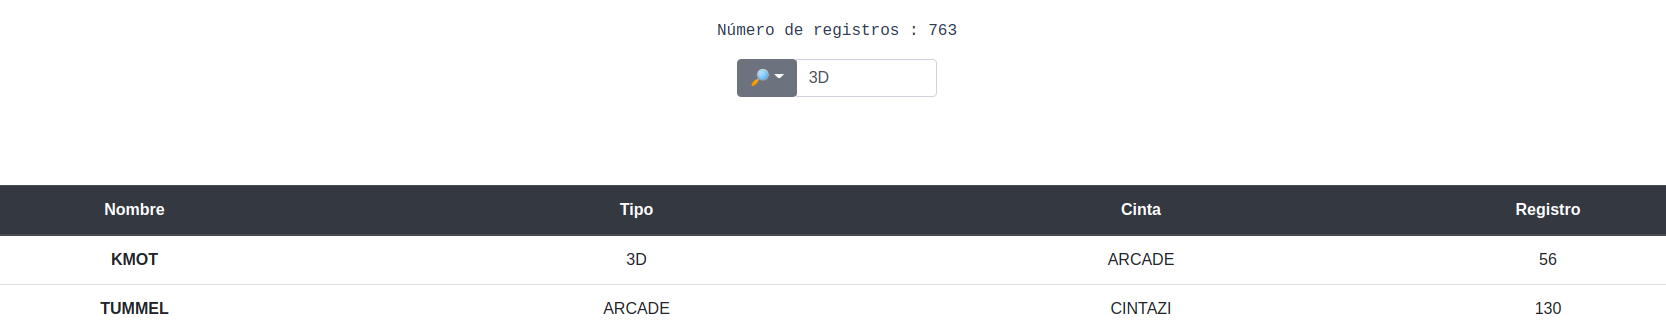
\includegraphics[scale=0.4]{images/cap_legados_web.png}
\caption{Captura de pantalla de la interfaz web}
\label{fig:aplicacion_legada_web}
\end{figure}
\newpage
Para integrar este \emph{frontend} con el código del servidor de \emph{backend} se ha creado un \emph{script BASH} para compilar y copiar el resultado de este proyecto al servidor \emph{backend}. El código del \emph{script} es el mostrado en el código \ref{list:copyToTomcat}.

\lstinputlisting[language=sh, label=list:copyToTomcat]{listings/copyToTomcat.sh}

\subsection{Backend del Wrapper}
El lenguaje utilizado para la realización de la práctica ha sido \textit{Java}, ya que, además de ser un lenguaje muy flexible y cómodo para los integrantes del grupo, se tiene experiencia con las herramientas que se utilizarán durante el desarrollo de la práctica.\\
%{\Huge \textbf{Esto es redundante porque se ha comentado en el apartado de \emph{Tecnología elegida}.}}\\

Para la realización de la parte del \textit{Backend} se ha utilizado el \textit{framework SpringBoot}. Se ha escogido esta tecnología principalmente debido a que \textit{Spring} incluye un servidor \textit{apache Tomcat}, lo que facilita mucho su configuración y despliegue. Para la integración de \textit{Spring} se ha utilizado \textit{Gradle}, un gestor de dependencias simple y fácil de utilizar que se ha utilizado anteriormente en otras asignaturas.\\
%\textbf{COMENTAR ALGO MÁS DE LAS TECNOLOGÍAS?}\\

Como se ha mencionado anteriormente, se expone una \textit{API REST} mediante la cual el cliente puede acceder a distintos recursos proporcionados por el servidor a través de las opciones que se muestran en la página principal. Para ello, se han creado tres \textit{endpoints}:
\begin{itemize}
	\item \textit{/filterByName}: Obtiene todos los registros cuyo nombre coincide con el nombre que se le pasa como parámetro.
	\item \textit{/filterByTape}: Obtiene todos los registros que pertenecen a la tapa cuyo nombre se pasa como parámetro.
	\item \textit{/getRecords}: Obtiene el número de registros almacenados en la aplicación.
\end{itemize}
Para poder abrir el emulador desde la aplicación se ha utilizado el comando \textit{dosbox}, el cual se es inicializado en cada llamada a la \textit{API REST} mediante el comando \textit{ProcessBuilder}.  Al final de cada llamada, el proceso es destruido mediante el comando \textit{destroy}. Tras ser llamado, se realiza una espera de 5 segundos para que todo el proceso se inicie de forma correcta.\\

La comunicación entre el servidor y el programa \textit{DosBox} se realiza mediante la clase \textit{Robot} de \textit{Java} (java.awt.Robot). De esta manera se permite generar eventos de ratón y teclado en el servidor, comunicándose de esta manera con el emulador \textit{DosBox}. El problema de la clase \textit{Robot} es que utiliza una objetos de tipo \textit{Key} para realizar las distintas acciones. Para poder indicar a la clase \textit{Robot} la acción a realizar en función de la tecla o acción de ratón utilizada, se ha creado otra clase llamada \textit{RobotAdapter} inspirada en un código encontrado en la web.\footnote{\url{https://stackoverflow.com/questions/1248510/convert-string-to-keyevents}}\\

\subsubsection{Problemas con el OCR}

Para obtener y procesar la respuesta del emulador, se utiliza \textit{Tesseract}, una herramienta de reconocimiento de caracteres (\textit{OCR}). Inicialmente se ha utilizado el \textit{dataset} adjuntado con los archivos de la práctica, el cual no reconocía correctamente algunos caracteres, por lo que se decidió probar otro conjunto de datos de entrenamiento para observar si existía una mejora en los resultados. Se utilizó un \textit{dataset} obtenido de \textit{Github}\footnote{\url{https://github.com/tesseract-ocr/tessdata/blob/master/spa.traineddata}}, con el cual se obtuvieron peores resultados que con el inicial, por lo que finalmente se utilizó el conjunto proporcionado con los archivos de la práctica. Aún así, algunas palabras y caracteres no son reconocidas de forma correcta por el \textit{OCR}, por lo que los resultados pueden ser erróneos en ocasiones. \\
Para indicar al objeto de la clase \textit{OCR} el lugar en la pantalla que debe procesar, se ha utilizado el comando \textit{wmctrl}, el cual obtiene la posición exacta de cada una de las ventanas que aparecen en el escritorio en el momento de su invocación. Para obtener la de la aplicación \textit{DosBox}, se utiliza el comando \textit{wmctrl} mediante \texttt{ProcessBuilder(WMCTRL\_PATH, "-lG")} y se analiza la salida producida con \textit{BufferReader}.De esta manera se obtiene las coordenadas \textit{x} e \textit{y} las cuales se utilizan para crear un objeto de tipo \textit{BufferedImage} mediante una función de la clase \textit{Robot} \texttt{robot.createScreenCapture}. Este objeto es analizado por el \textit{OCR} mediante la función \texttt{ocr.doOCR}, la cual devuelve el contenido de la imagen en formato \textit{String}.\\

Como el reconocimiento de carácteres no es perfecto se probaron otras alternativas, aunque sin éxito para tratar de mejorar la precisión del mismo. Se probó el invertir los colores de la imagen para obtener el fondo blanco y el texto en negro. También se trató de binarizar los colores de las imágenes a blanco y negro puro y no el gris que se utiliza en la terminal. Ninguna de estas opciones dieron buenos resultados.\\
Se intentó utilizar otra herramienta de reconocimiento de caracteres. La herramienta era \emph{Asprise OCR\footnote{\url{https://asprise.com/royalty-free-library/java-ocr-api-overview.html}}}. Esta herramienta en su versión de prueba sustituye los caracteres \emph{q,x,0,9} por un asterisco (\emph{*}). Tras intentar utilizar esta herramienta, creando una interfaz \emph{OCRInterface} para la unificación de opciones.\\

Tras la derrota en el campo del OCR se planteó el uso de otro emulador de \emph{MSDOS} para intentar leer la salida estándar del programa y evitar el uso de OCR. Se probó \emph{dosemu\footnote{\url{http://www.dosemu.org/}}}. Este emulador tiene la característica de poder utilizar la terminal como una \emph{``dumb terminal''} con la opción \emph{-dumb}. Con esta opción el programa legado no funcionaba ya que no es una aplicación que escriba en la salida estándar.\\
Con la opción \emph{-t} el emulador funciona como \emph{-dumb} pero utilizando colores\footnote{\textbf{\url{https://retrocomputing.stackexchange.com/questions/16173/emulate-a-text-mode-dos-program-using-a-unix-terminal}}}. Desde una terminal haciendo las pruebas manualmente parecía funcionar pero luego, llevado a la implementación en \emph{Java} no. Ocurría lo mismo que con la opción \emph{-dumb}, aparecía una sola línea en la salida estándar que mostraba:

\begin{lstlisting}
C:\Database\>gwbasic.exe database
\end{lstlisting}

Se buscaron soluciones en distintos foros como \href{https://www.vogons.org/viewtopic.php?t=36268}{Vogons}, aunque ninguna de las soluciones propuestas resultó de utilidad. Otra de las \href{https://www.reddit.com/r/dosbox/comments/bvoij9/piping_dosboxs_output_to_stdout_and_stderr/}{soluciones} propuestas indicaba que se utilizara la opción \textit{- noconsole} de \textit{DOSBox} para Windows, con la que tampoco se consiguió redirigir la salida.

En resumen, la única solución funcional ha consistido en el uso del OCR la cual, aunque no reconoce correctamente el 100\% de los caracteres, podemos obtener la salida del emulador desde el programa en Java.



\end{document}